\section{Introducción}
\subsection{UCTP}
La asignación automática de horarios académicos, conocida como University Course Timetabling Problem (UCTP), es un problema clásico de optimización combinatoria 
presente en instituciones educativas de todos los niveles. Consiste en asignar, de manera eficiente, cursos, grupos, salones y franjas horarias, respetando un 
conjunto de restricciones duras (hard constraints), tales como evitar traslapes de clases, asignacion de salones adecuados o disponibilidad de espacios, así como 
restricciones blandas (soft constraints), que buscan mejorar la calidad del horario, como minimizar demasiadas horas consecutivas, distribuir las clases durante la semana 
o evitar largos periodos sin actividad.

El UCTP es un problema NP-hard debido al gran número de combinaciones posibles y a la interacción compleja entre todas las restricciones, lo que hace inviable una solución 
óptima mediante métodos exhaustivos. Por ello, se han adoptado algoritmos metaheurísticos capaces de explorar grandes espacios de búsqueda de manera eficiente. 
Entre ellos, los Algoritmos Genéticos (AG) han demostrado ser una herramienta robusta para encontrar soluciones de alta calidad en tiempos razonables.

Los AG se inspiran en los mecanismos de la evolución biológica, operando con una población de posibles soluciones (individuos) que evolucionan a través de operadores 
como selección, cruce y mutación. En el contexto del UCTP, cada individuo representa un horario completo con todas las materias asignadas y su calidad se evalúa mediante 
una función de aptitud que penaliza el incumplimiento de restricciones. A través de múltiples generaciones, el algoritmo incrementa la viabilidad y calidad de los 
horarios generados, permitiendo obtener soluciones que cumplen con las restricciones duras y optimizan las blandas.

Abordaremos una implementación del UCTP utilizando un Algoritmo Genético diseñado para manejar múltiples planes de estudio, diversos tipos de salones y 
diferentes duraciones de clase. Además, se incorporan mecanismos adicionales como verificación de compatibilidad de salones, penalización de cruces, 
control de consecutividad máxima de clases y exportación automatizada de los horarios en formato Excel para su inspección. Este enfoque permite generar horarios 
completos y coherentes ajustados a las necesidades reales de operación académica.

\subsection{Cursos Considerados}
Para este problema nos enfocaremos en 4 cursos diferentes los cuales son:

\begin{itemize}\label{cursos}
	\item Maestria en Ciencias en Inteligencia Artificial.
	\item Ingenieria Fisica.
	\item Ingenieria en Nanotecnologia.
	\item Ingenieria en Biomedica.
\end{itemize}

En este caso cada curso cuenta con su propio plan de estudio, pero todas comparten los mismos salones disponibles asi como los laboratorios, ademas de que en algunos casos
aunque las materias sean las mismas, se deben impartir por curso no solo una vez, por lo cual tambien se toma en cuenta que el tamaño de los grupos corresponda con el cupo
del salon.

\subsection{Consideraciones}

Para este ejercicio se tomaron como referencia los salones disponibles en el Campus Aereopuerto de la UAQ y que una vez que se recolecto la informacion de los salones se 
obtuvo lo siguiente:

\begin{figure}[H]
    \centering
    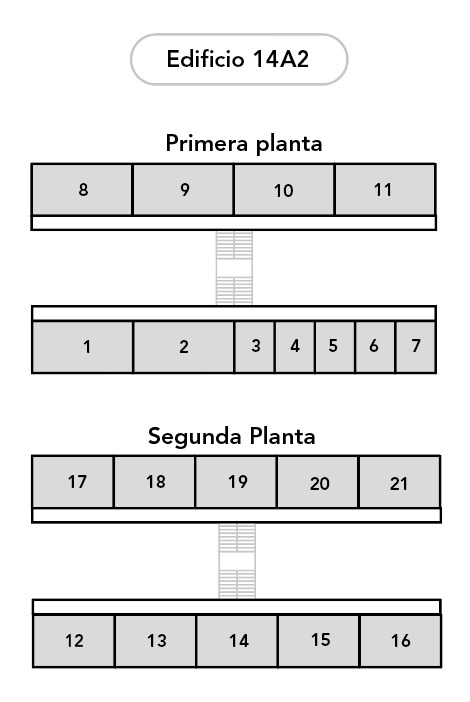
\includegraphics[width=0.25\textwidth]{rsc/img/intro/Edificio_14A2.jpeg}
    \caption{Salones Disponibles en el Edificio 14A2}\label{fig: Edificio_14A2}
\end{figure}

\begin{figure}[H]
    \centering
    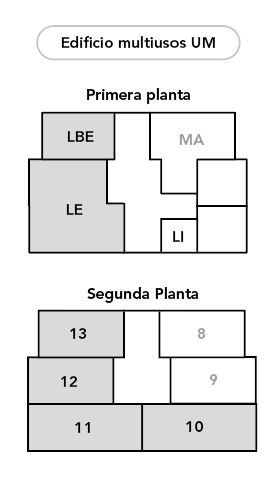
\includegraphics[width=0.25\textwidth]{rsc/img/intro/UM.jpeg}
    \caption{Salones Disponibles en el Edificio de Usos Multiples}\label{fig: Edificio_UM}
\end{figure}

Como podemos ver en el Edificio 14A2 (Figura~\ref{fig: Edificio_14A2}) existen salones más pequeños los cuales se deben tomar en cuenta debido a su cupo. Por otro lado en el Edificio de 
Usos Multiples (Figura~\ref{fig: Edificio_UM}) es donde existen dos de los laboratorios disponibles, sin embargo despues de analizar el plan de estudios de los diferentes 
cursos se tomo la libertad de crear un laboratorio extra de Quimica para las carreras que lo necesiten, este laboratorio si existe, simplemente se encuentra en otro edificio.